\documentclass{article}

\def\TemplatePath{../}

%%% Template Packages %%%

\usepackage{xifthen} % Template stuff 
\usepackage{graphicx} % Images
\usepackage{tcolorbox} % Color Box
\usepackage[%
vmargin=2cm,%
hmargin=2.25cm,%
headheight=22pt%
]{geometry} % Page Geometry
\usepackage{fancyhdr} % Header / Footer Styles
\usepackage{extramarks} % Header / Footer Marks

\usepackage{ragged2e} % Text Align
\usepackage{amsmath} % Math Align

\usepackage{booktabs} % Tables+ Package
\usepackage[inline]{enumitem} % Enumarete+ Package
\usepackage{multicol} % Fancier Enumaretes++ Package
\usepackage{xparse} % Command Args Split Package

\usepackage{mathtools} % Math General
\usepackage{amsthm} % Math Envs
\usepackage{unicode-math} % Math Symbols

\usepackage{polyglossia} % Language
    \setdefaultlanguage{spanish}%

%%% Variables and Such %%%
\ifthenelse{\isundefined{\TemplatePath}}{%
    \def\TemplatePath{template/}
}{}

%%% Template Styles %%%

% Header / Footer Styles
\pagestyle{fancy}
\RenewDocumentCommand{\headrule}{}{%
    \rule[0.1cm]{\textwidth}{0.1mm}%
}

\ifthenelse{\isundefined{\MyTitle}}{}{%
\fancyhf[HC]{{\slshape \MyTitle{}}}
}%
\fancyhead[HL]{\firstleftxmark}
\fancyhead[HR]{\lastleftxmark}

\RenewDocumentCommand{\footrule}{}{%
    \rule[0.1cm]{\textwidth}{0.1mm}%
}

\renewcommand{\thefootnote}{\Roman{footnote}} % Changing footnotes arabic to roman numbers

% Redefine \maketitle
\RenewDocumentCommand{\maketitle}{s}{%
    \begin{@twocolumntrue}%
        \begin{minipage}{0.3\textwidth}%
            \begin{Center}
                \includegraphics[width=0.5\textwidth]{\TemplatePath src/unal_logo.pdf}%
            \end{Center}
        \end{minipage}%
        \begin{minipage}{0.7\textwidth}{%
            \begin{Center}
                \ifthenelse{\isundefined{\MyClass}}{%
                    {\large Set \textbackslash{}def\textbackslash{}MyClass\{your\_class\} in the preamble} \\[0ex]%
                }{%

                    {\large \itshape \MyClass{}} \\[0.75ex]
                }%
                \ifthenelse{\isundefined{\MyTitle}}{%
                    {\huge Set \textbackslash{}def\textbackslash{}MyTitle\{doc\_title\} in the preamble} \\[4ex]%
                }{%
                    {\huge \slshape \MyTitle{}} \\[1.5ex]%
                }%
                \ifthenelse{\isundefined{\MyAuthor}}{%
                    {\Large Set \textbackslash{}def\textbackslash{}MyAuthor\{your\_name\} in the preamble} \\%
                }{%
                    {\Large \MyAuthor{}} \\%
                }%
                \ifthenelse{\isundefined{\MyEmail}}{%
                    {\small Set \textbackslash{}def\textbackslash{}MyEmail\{your\_email\} in the preamble} \\[4ex]%
                }{%
                    {\small \MyEmail{}} \\[1ex]%
                }%
                \ifthenelse{\isundefined{\MyDate}}{%
                    Set \textbackslash{}def\textbackslash{}MyDate\{doc\_date\} in the preamble%
                }{%
                    \MyDate{}%
                }%
            \end{Center}
        }%
        \end{minipage}%
    \end{@twocolumntrue}%
    \vspace{0.25cm}%
    \begin{Center}%
        \rule[0cm]{\textwidth}{0.1mm}%
    \end{Center}%
}

% Enumerate Lists types
\newcommand\SetItemnumber[1]{\setcounter{enumi}{\numexpr#1-1\relax}}
\newcommand{\listSubscript}[2]{\(#1_{#2}\)}
\newcommand{\listAlp}{\alph*.}
\newcommand{\listALPH}{\Alph*.}

% Fast Supper and Sub -scripts
\NewDocumentCommand{\tsup}{m} {\textsuperscript{#1}}
\NewDocumentCommand{\tsub}{m} {\textsubscript{#1}}

% Set of Numbers
\def\realR{\symbb{R}} % Real
\def\realN{\symbb{N}} % Natural
\def\realZ{\symbb{Z}} % Integers
\def\realQ{\symbb{Q}} % Rational
\def\realC{\symbb{C}} % Complex
\def\realC{\symbb{I}} % Irrational

%%% Template Math stuff %%%

% Cases and stuff
\newtheorem{TMPMathCases}[]{Caso}
\NewDocumentCommand{\ResetCases}{} {\setcounter{TMPMathCases}{0}}
\NewDocumentEnvironment{mathcase}{O{}m} {%
    \IfValueTF{#1}{%
        \begin{TMPMathCases}[#1] % 
            #2%
        \end{TMPMathCases}%
    }{%
        \begin{TMPMathCases} % 
            #2%
        \end{TMPMathCases}%
    }
} {}

% Definitions
\newtheorem{TMPMathDefinition}{Definición}
\NewDocumentEnvironment{definition}{+b} {%
    \begin{tcolorbox}[left=0mm,right=0mm]%
        \begin{TMPMathDefinition}%
            #1 %
            \hspace{\fill}\(\bigtriangleup\)%
        \end{TMPMathDefinition}%
    \end{tcolorbox}%
} {}

% Fast Function
\NewDocumentCommand{\ffunc}{mm} {%
    #1\left(#2\right)
}

% Fast Set
\NewDocumentCommand{\fset}{m} {%
    \left\{%
        #1 %
    \right\}%
}

% Fast Image 
\NewDocumentCommand{\fim}{m} {%
    \text{Im}\left(%
        #1%
    \right)%
}

% Fast Power Set
\NewDocumentCommand{\fps}{m} {%
    \symscr{P}\left(%
        #1%
    \right)%
}

% Fast Cardinal
\NewDocumentCommand{\fcard}{m} {%
    \left|#1\right|
}


\usepackage{biblatex}
    \addbibresource{./references.bib}

\usepackage{tikz}
    \usetikzlibrary{calc}

\definecolor{area}{rgb}{0.6,0.4,0.8}

\def\MyClass{Introducción a la Teoria de Conjuntos}
\def\MyTitle{Hrbacek, Jech-Ejercicios}
\def\MyAuthor{Martín Steven Hernández Ortiz}
\def\MyEmail{mahernandezor@unal.edu.co}
\def\MyDate{\today}

\newcommand{\fp}{\symscr{P}}

\begin{document}
\maketitle{}
Ejercicios tomados de la sección 1 del capitulo 4, en el libro~\cite{hrbacek_introduction_1999}.

\begin{definition}
    Una función \(F: \fps{A} \rightarrow \fps{A}\) es \textbf{monótona} 
    si \(X \subseteq Y \subseteq A\) implica que \(F(X) \subseteq F(Y)\).
\end{definition}
\begin{definition}
    Para una función \(F: \fps{A} \rightarrow \fps{A}\), 
    \(X \subseteq A\) es un \textbf{punto fijo de \(F\)} si \(F(X) = X\).
\end{definition}
\begin{enumerate}[label=1.\arabic*,start=10,ref=(1.\arabic*)]
    \item Sea \(F: \fps{A} \rightarrow \fps{A}\), una función monótona. Entonces \(F\) tiene un punto fijo. \\
    Primero, sea \(T = \fset{ X \subseteq A : F(X) \subseteq X}\). Note que \(T \neq \emptyset\), ya que \(A \in T\).
    Ahora, sea \(\hat{X} = \cap T\), entonces para todo \(t \in T\) se tiene que \(\hat{X} \subseteq t \subseteq A\),
    como \(F(t) \subseteq t\), y como \(F\) es monótona \(F(\hat{X}) \subseteq F(t)\), 
    luego \(F(\hat{X}) \subseteq F(t) \subseteq \hat{X} \subseteq t\), es decir \(F(\hat{X}) \subseteq \hat{X}\) y \(\hat{X} \in T\).
    Ahora, de manera similar, \(F(\hat{X}) \subseteq \hat{X} \subseteq A\), entonces \(F(F(\hat{X})) \subseteq F(\hat{X})\) y \(F(\hat{X}) \in T\).
    Como \(\hat{X} = \cap T\), entonces \(\hat{X} \subseteq F(\hat{X})\), pero como \(F(\hat{X}) \subseteq \hat{X}\), 
    se tiene que \(\hat{X} = F(\hat{X})\), donde \(\hat{X} \in A\).\qed{}
\label{pt1_10}
    \item Usando el ejercicio~\ref{pt1_10}, pruebe el \emph{Teorema de Cantor-Bernstein}. \\
    Debemos probar que si \(\fcard{X} < \fcard{Y}\) y \(\fcard{Y} < \fcard{X}\) entonces \(\fcard{X} = \fcard{Y}\). 
    Sean \(f: X \rightarrow Y\) y \(g: Y \rightarrow X\), funciones inyectivas.
    Primero, considere \(g \circ f: X \rightarrow X\), luego \((g \circ f)(X) \subseteq g(Y) \subseteq X\), y note que \(\fcard{X} = \fcard{(g \circ f)(X)}\) y \(\fcard{Y} = \fcard{g(Y)}\).
    Vamos a notar \(A = X\), \(A_1 = (g \circ f)(X)\) y \(B = g(Y)\). \\
    Ahora, Sean \(\overline{f}: A \rightarrow A_1\) una función biyectiva, y \(F: \fps{A} \rightarrow \fps{A}\) una función, 
    definida como \(x \mapsto (A - B) \cup \overline{f}(x)\), veamos que \(F\) es monótona.
    Como \(A_1 \subseteq B \subseteq A\),
    veamos para un \(a \in F(A)\) cualquiera, entonces 
    \[
        \begin{aligned}
            &\phantom{\Rightarrow} a \in (A - B) \cup \overline{f}(A_1) \\
            &\Rightarrow a \in (A - B) \vee a \in \overline{f}(A_1) \\
            &\Rightarrow (a \in A \wedge a \not\in B) \vee (a \in \overline{f}(A_1))
        \end{aligned}
    \]
    Si \(a \in A\) y \(a \not\in B\), entonces \(a \in (A - B) \cup \overline{f}(B) = F(B)\).
    Si \(a \in \overline{f}(A_1)\), como \(A_1 \subseteq B\), entonces \(\overline{f}(A_1) \subseteq \overline{f}(B)\), 
    y \(a \in (A - B) \cup \overline{f}(B) = F(B)\). Concluyendo que \(F(A_1) \subseteq F(B)\). \\
    Como \(F\) es monótona, por~\ref{pt1_10} tiene un punto fijo \(C \subseteq A\), tal que \(F(C) = (A - B) \cup \overline{f}(C) = C\), y sea \(D = A - C\), 
    definamos a \(G: A \rightarrow B\), como 
    \[
        G(x) = 
        \begin{cases}
            \overline{f}(x) & \text{Si } x \in C \\
            x & \text{Si } x \in D
        \end{cases}
    \]
    Primero, veamos que \(G \upharpoonright C\) es una función inyectiva. Sean \(x, x' \in C\) tales que \(G(x) = G(x')\), 
    entonces \(G(x) = \overline{f}(x) = \overline{f}(x') = G(x')\), como \(\overline{f}\) es inyectiva, se tiene que \(x = x'\).
    Ahora, veamos que \(G \upharpoonright D\) es una función inyectiva también. Sean \(x, x' \in D\) tales que \(G(x) = G(x')\),
    entonces \(G(x) = x = x' G(x')\). \\
    Como \(G \upharpoonright C\) y \(G \upharpoonright D\) son inyectivas, para que \(G\) también sea inyectiva, 
    se debe tener que \(\fim{G \upharpoonright C} \cap \fim{G \upharpoonright D} = \emptyset\). Asuma que \(\fim{G \upharpoonright C} \cap \fim{G \upharpoonright D} \neq \emptyset\),
    entonces existe \(y \in \fim{G \upharpoonright C} \cap \fim{G \upharpoonright D}\), 
    tal que existen \(x \in C\) y \(x' \in D\) tales que \(G(x) = \overline{f}(x) = y = x' = G(x')\).
    Pero antes, note que \(x' \in D = A - C\), entonces 
    \[
        \begin{aligned}
            &\phantom{\Rightarrow} x' \in A - \left((A - B) \cup \overline{f}(C)\right) \\
            &\Rightarrow \left(x' \in \left(A - (A - B)\right)\right) \wedge \left(x' \in \left(A - \overline{f}(C)\right)\right) \\
            &\Rightarrow \left(x' \in (A - A) \vee x' \in (A \cap B)\right) \wedge \left(x' \in \left(A - \overline{f}(C)\right)\right) \\
            &\Rightarrow x' \in B \cap (A - \overline{f}(C)) \\
            &\Rightarrow x' \in B - \overline{f}(C)
        \end{aligned}
    \]
    Esto se tiene ya que \(\overline{f}(C) \subseteq A_1 \subseteq B \subseteq A\).
    Luego, \(x' = y \not\in \overline{f}(C)\), pero \(y = \overline{f}(x) \in \overline{f}(C)\); Absurdo. 
    Entonces no existe puede existir \(y\) y \(\fim{G \upharpoonright C} \cap \fim{G \upharpoonright D} = \emptyset\), es decir, \(G\) es inyectiva. \\
    Ahora, veamos que \(G\) es sobreyectiva. Entonces, debemos probar que \(\fim{G \upharpoonright C} \cup \fim{G \upharpoonright D} = B\)
    \[
        \begin{aligned}
            \fim{G \upharpoonright C} \cup \fim{G \upharpoonright D}
                &= \overline{f}(C) \cup D \\
                &= \overline{f}(C) \cup \left(B - \overline{f}(C)\right) \\
                &= B
        \end{aligned}
    \]
    Concluyendo que \(G\) es una biyección entre \(A = X\) y \(B = g(Y)\), es decir \(\fcard{X} = \fcard{Y}\).\qed{}
\label{pt1_11}
    \item Puebe que el punto fijo del ejercicio~\ref{pt1_10}, \(\hat{X}\), es el menor punto fijo de \(F\), 
    es decir, si \(F(X) = X\) para algún \(X \subseteq A\), entonces \(\hat{X} \subseteq X\). \\
    Asuma que existe un punto fijo \(\ddot{X}\) de \(F\) tal que \(\ddot{X} \subseteq X\), para todo punto fijo \(X\) de \(F\),
    en especial \(\ddot{X} \subseteq \hat{X} = \cap\left\{X \subseteq A: F(X) \subseteq X\right\}\), sin embargo, 
    como \(F(\ddot{X}) = \ddot{X} \Rightarrow F(\ddot{X}) \subseteq \ddot{X}\), entonces \(\ddot{X} \in \left\{X \subseteq A: F(X) \subseteq X\right\}\).
    Luego, \(\hat{X} \subseteq \ddot{X}\), es decir \(\ddot{X} = \hat{X}\).\qed{}

\label{pt1_12}
\end{enumerate}
\begin{definition}
    Una función \(F: \fps{A} \rightarrow \fps{A}\) es \textbf{continua} si \(F\left(\bigcup_{i \in \omega} X_i\right) = \bigcup_{i \in \omega} F(X_i)\)
    para cualquier secuencia no-decreciente de subconjuntos de \(A\), \(\left\langle X_k \subseteq A: k \in \omega \right\rangle\), 
    donde si \(i \leq j\) entonces \(X_i \subseteq X_j\)
\end{definition}
\begin{enumerate}[label=1.\arabic*,start=13,ref=(1.\arabic*)]
    \item Pruebe que la función \(F\) usada en el ejercicio~\ref{pt1_11} es continua. \\
    Primero probemos que para una función \(f\) cualquiera, \(f\left(\cup_{a \in A} X_a\right) = \cup_{a \in A} f\left(X_a\right)\).
    Sea \(y \in f\left(\cup_{a \in A} X_a\right)\), entonces existe \(x \in \cup_{a \in A} X_a\) tal que \(f(x) = y\), 
    luego existe \(a \in A\) tal que \(x \in X_a\), es decir existe \(a \in A\) tal que \(y \in f(X_a)\), lo que es equivalente a
    \(\cup_{a \in A} f(X_a)\). Si \(y \in \cup_{a \in A} f(X_a)\) se puede seguir un argumento similar. 
    Probando que \(f\left(\cup_{a \in A} X_a\right) = \cup_{a \in A} f\left(X_a\right)\). \\
    Ahora, para que \(F\) sea continua se debe probar que para cualquier secuencia no-decreciente de subconjuntos de \(A\) se debe tener que
    \[
        \begin{aligned}
            F\left(\bigcup_{n \in \omega} X_n\right) 
                &= (A - B) \cup f\left(\bigcup_{n \in \omega} X_n\right) \\
                &= (A - B) \cup \bigcup_{n \in \omega} f\left(X_n\right) \\
                &= \bigcup_{n \in \omega} \left((A - B) \cup f\left(X_n\right)\right) \\
                &= \bigcup_{n \in \omega} F\left(X_n\right)
        \end{aligned}
    \]
    Entonces \(F\) es una función continua.\qed{}

\label{pt1_13}
    \item Pruebe que si \(\hat{X}\) es el menor punto fijo de una función monótona y continua, \(F: \fps{A} \rightarrow \fps{A}\), 
    entonces \(\hat{X} = \bigcup_{i \in \omega} X_i\), donde se define recursivamente \(X_0 = \emptyset, X_{i+1} = F(X_i)\). \\
    Primero, veamos que la sucesión \(S = \left\langle X_i \subseteq A: i \in \omega \right\rangle\) es no-decreciente mediante inducción sobre \(i\).
    \vspace{-1ex}
    \begin{enumerate}
        \item[(0)] \(X_0 = \emptyset \subseteq X_i\) para todo \(i \in \omega\).
        \item[\((n \Rightarrow n + 1)\)] Asuma que \(X_n \subseteq X_{n+1} = F(X_n)\), veamos que 
            \(X_{n + 1} = F(X_n) \subseteq F(X_{n+1}) = X_{n+2}\) ya que \(F\) es monótona. Entonces \(X_{i} \subseteq X_{i + 1}\) para todo \(i \in \omega\).
    \end{enumerate}
    Concluimos que la sucesión \(S\) es no-decreciente, entonces \(F\) va a ser continua para \(S\). 
    Ahora, veamos que \(\ddot{X} = \cup_{i \in \omega} X_i\) es un punto fijo de \(F\)
    \[
        \begin{aligned}
            F(\bigcup_{i \in \omega} X_i) 
                &= \bigcup_{i \in \omega} F(X_i) \\
                &= F(X_0) \cup F(X_1) \cup F(X_2) \cup \cdots \\
                &= X_1 \cup X_2 \cup X_3 \cup \cdots \\
                &= \bigcup_{i \in \omega} X_i
        \end{aligned}
    \]
    Ahora, veamos que \(\ddot{X}\) es el menor punto fijo de \(F\). 
    Para eso debemos probar que para todo \(i \in \omega\), se tenga que \(X_i \subseteq X\),
    donde \(X\) es un punto fijo cualquiera de \(F\), probemos esto mediante inducción sobre \(i\).
    \vspace{-1ex}
    \begin{enumerate}
        \item[(0)] \(X_0 = \emptyset \subseteq X\).
        \item[\((n \Rightarrow n + 1)\)] Asuma que \(X_n \subseteq X \subseteq A\), luego como \(F\) es monótona, 
            \(F(X_n) = X_{n+1} \subseteq F(X)\), y como \(X\) es un punto fijo, entonces \(X_{n+1} \subseteq X\).
    \end{enumerate}
    Entonces \(\ddot{X} = \bigcup_{i \in \omega} X_i \subseteq X\).
    Note que si \(\hat{X}\) es también el menor punto fijo de \(F\), entonces \(\hat{X} \subseteq \ddot{X}\) y \(\ddot{X} \subseteq \hat{X}\), 
    es decir \(\hat{X} = \ddot{X} = \bigcup_{i \in \omega} X_i\).\qed{}
\label{pt1_14}
    %\item[(extra)] Compare la prueba del \emph{Lemma \(1.7\)} usado para probar el \emph{Teorema de Cantor-Bernstein} en~\cite{hrbacek_introduction_1999} 
    con la construcción del menor punto fijo, \(\hat{X}\), de \(F(X) = (A - B) \cup \overline{f}(X)\) en el ejercicio~\ref{pt1_14}. \\
    Si construyeramos el menor punto fijo \(\hat{X}\) de \(F\), como se hizo en el ejercicio~\ref{pt1_14}. 
    Veamos algunos terminos de la sucesión \(S\) de subconjuntos de \(A\) 
    \[
        \begin{aligned}
            X_0 &= \emptyset \\
            X_1 &= F(X_0) = (A - B) \cup \overline{f}(\emptyset) = (A - B) \\
            X_2 &= F(X_1) = (A - B) \cup \overline{f}(X_1) = (A - B) \cup \overline{f}((A - B)) \\
            X_3 &= F(X_2) = (A - B) \cup \overline{f}(X_2) = (A - B) \cup \overline{f}((A - B) \cup \overline{f}((A - B))) \\
            & \hspace{0.5ex} \vdots \\
            X_{i + 1} &= F(X_i) = (A - B) \cup \overline{f}(X_i)
        \end{aligned}
    \]
    Primero, note que no es tan fácil de ver que esta pasando dentro de \(\overline{f}\) para cada iteración de \(i\).
    Creo que es mejor mirar un dibujo sobre los terminos de \(S\). 
    \\[0.5cm]
    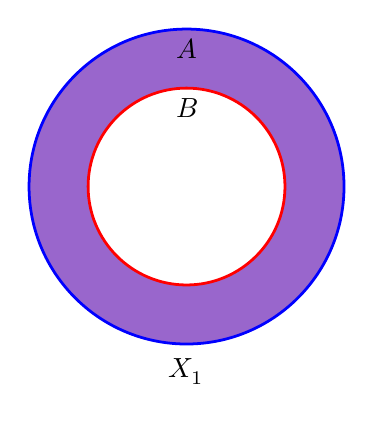
\begin{tikzpicture}
        \draw[blue,line width=1, fill=area] (0,0) circle[radius=2] (0, 1.75) node[black] {\(A\)};
        \draw[red,line width=1, fill=white] (0,0) circle[radius=1.25] (0, 1) node[black] {\(B\)};
        \draw (0,-2.35) node {\(X_1\)};
    \end{tikzpicture}
    \hspace{0.5cm}
    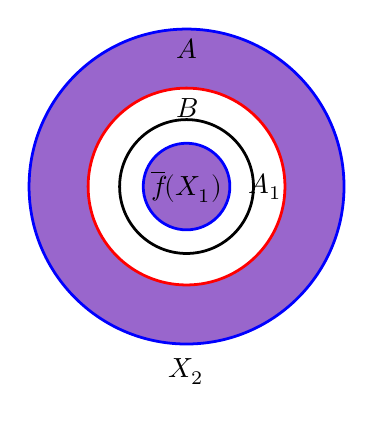
\begin{tikzpicture}
        \draw[blue,line width=1, fill=area] (0,0) circle[radius=2] (0, 1.75) node[black] {\(A\)};
        \draw[red,line width=1, fill=white] (0,0) circle[radius=1.25] (0, 1) node[black] {\(B\)};
        \draw[black,line width=1, fill=white] (0,0) circle[radius=0.85] (1, 0) node[black] {\(A_1\)};
        \draw[blue,line width=1, fill=area] (0,0) circle[radius=0.55] (0, 0) node[black] {\(\overline{f}(X_1)\)};
        \draw (0,-2.35) node {\(X_2\)};
    \end{tikzpicture}
    \hspace{0.5cm}
    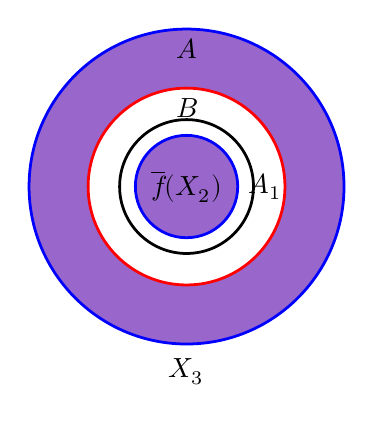
\begin{tikzpicture}
        \draw[blue,line width=1, fill=area] (0,0) circle[radius=2] (0, 1.75) node[black] {\(A\)};
        \draw[red,line width=1, fill=white] (0,0) circle[radius=1.25] (0, 1) node[black] {\(B\)};
        \draw[black,line width=1, fill=white] (0,0) circle[radius=0.85] (1, 0) node[black] {\(A_1\)};
        \draw[blue,line width=1, fill=area] (0,0) circle[radius=0.65] (0, 0) node[black] {\(\overline{f}(X_2)\)};
        \draw (0,-2.35) node {\(X_3\)};
    \end{tikzpicture}
\label{ptextra}
\end{enumerate}
    \printbibliography{}
\end{document}
